\documentclass[10pt,a4paper,twocolumn]{IEEEtran}
\usepackage[latin1]{inputenc}
\usepackage{amsmath}
\usepackage{amsfonts}
\usepackage{amssymb}
\usepackage{graphics}
\author{
Himani bhatt \hspace{38pt} Janvi Shah \and \hspace{35pt} \and Priyanka Nimavat \hspace{35pt} \and Sahil Desai\\
1421003 \hspace{60pt} 1421004 \hspace{55pt}
1421010 \hspace{65pt} 1421014\\
IET AU \hspace{60pt} IET  AU \hspace{60pt} IET AU \hspace{65pt} IET AU \\
\small
himanibhatt8@gmail.com \hspace{10pt} shahjanvi54@gmail.com \hspace{10pt} priyanka.m@gmail.com \hspace{10pt} sahilzdesai@gmail.com }
\title{Survey Report On Face Detection}
\begin{document}
\maketitle
\begin{abstract}
Face detection has been one of the most studied topics in the computer vision literature. In this technical report, we survey the recent advances in face detection for the past decade. We survey the various techniques according to how they extract features and what learning algorithms are adopted. It is our hope that by reviewing the many existing algorithms, we will see even better algorithms developed to solve this fundamental computer vision problem.\\
Keywords:

\end{abstract}
\begin{IEEEkeywords}
Face Detection,Feature based approches
\end{IEEEkeywords}
\section{Introduction}

A face detector has to tell whether an image of arbitrary size contains a human face and if so, where it is. One natural framework for considering this problem is that of binary classification, in which a classifier is constructed to minimize the misclassification risk. Since no objective distribution can
describe the actual prior probability for a given image to have a face, the algorithm must minimize both the false negative and false positive rates in order to achieve an acceptable performance.
The challenges associated with face detection can be attributed to the following factors:
\begin{itemize}


\item \textbf{Pose} The images of a face vary due to the relative
camera-face pose (frontal, 45 degree, profile, upside
down), and some facial features such as an eye or the
nose may become partially or wholly occluded.
\item \textbf{Presence or absence of structural components.}
Facial features such as beards, mustaches, and glasses may or may not be present and there is a great deal of variability among these components including shape, color, and size.
\item \textbf{Facial expression.} The appearance of faces are directly affected by a person's facial expression.
\item \textbf{Occlusion.} Faces may be partially occluded by other objects. In an image with a group of people, some faces may partially occlude other faces.
\item \textbf{Image orientation.} Face images directly vary for different rotations about the camera's optical axis.
\item \textbf{Imaging conditions.} When the image is formed,factors such as lighting (spectra, source distribution and intensity) and camera characteristics (sensor response, lenses) affect the appearance of a face.
\end{itemize}
There are many techniques to detect a face. Here is a list of the most common approaches in face detection.
\begin{itemize}
\item Finding faces in images with controlled background: Use images with a plain monocolour background, or use them with a predefined static background - removing the background will always give you the face boundaries.
\item Finding faces by color:If you have access to color images, you might use the typical skin color to find face segments. The disadvantage: doesn't work with all kind of skin colors, and is not very robust under varying lighting conditions.
\item Finding faces by motion:If you are able to use real-time video, you can use the fact that a face is almost always moving in reality. Just calculate the moving area, and here you go. Disadvantages: What if there are other objects moving in the background?
\item Using a mixture of the above:Combining several good approaches normally yields an even better result.
\item Finding faces in unconstrained scenes:this is the main thing, the top of them all, the most complicated thing maybe in whole object recognition: Given a black and white still image, where is the face? Humans can do it, so where's the perfect algorithm that can do it, too?
Two mehods are:Model-based Face Tracking and Weak classifier cascades
\end{itemize}

\section{Methods}

Face detection can be divided into two approches:Feature-based approches and Image-based approches. These are further divded into many parts they are explained in Brief as follow.
\begin{itemize}
\item Feature-based approches
\begin{enumerate}
\item Low-level analysis
\begin{itemize}
\item \textbf{Edges}--Edges are those places in an image that correspond to object boundaries.
Edges are pixels where image brightness changes abruptly.
\item \textbf{Gray-levels}--The gray information within a face can also be used as features. Facial features such as eyebrows, pupils, and lips appear generally darker than their surrounding facial regions. This property can be exploited to differentiate various facial parts. The extraction of dark patches is achieved by low-level gray-scale thresholding. Local maxima, which are defined by a bright pixel surrounded by eight dark neighbors, are used instead to indicate the bright facial spots such as nose tips. When the resolution of a face image is reduced gradually either by subsampling or averaging, macroscopic features of the face will disappear. At low resolution, face region will become uniform.
\item \textbf{Color}-- One of the most widely used color models is RGB representation in which different colors are defined by combinations of red, green, and blue primary color components. Due to the extra dimensions that color has, two shapes of similar gray information might appear very differently in a color space. It was found that different human skin color gives rise to a tight cluster in color spaces even when faces of difference races are considered.
\item \textbf{Motion}--If the use of a video sequence is available, motion information is a convenient means of locating moving objects. A straightforward way to achieve motion segmentation is by frame difference analysis. In, moving frame that include face and body parts are extracted by thresholding accumulated frame difference.Another way of measuring visual motion is through the estimation of moving image contours.
\end{itemize}
\item Feature analysis
\begin{itemize}
\item \textbf{Feature Searching}--Feature searching techniques begin with the determination
of prominent facial features. The detection of the prominent features then allows for the
existence of other less prominent features to be hypothesized using anthropometric measurements
of face geometry. For instance, a small area on top of a larger area in a head and shoulder sequence implies a face on top of shoulder scenario, and a pair of dark regions found in the face area increase the confidence of a face existence.

\end{itemize}
\item active shape models
\begin{itemize}
\item \textbf{Snakes}--Active contours, or snakes, are commonly used to locate a head boundary. In order to achieve the task, a snake is first initialized at the proximity around a head boundary. It then locks onto nearby edges and subsequently assume the shape of the head.Two main considerations in implementing a snake are the selection of the appropriate
energy terms and the energy minimization technique.
\item \textbf{Deformable templates}--Use the concept of snakes a step further by incorporating global information of the eye to improve the reliability of the extraction process. The deformation mechanism involves the steepest gradient descent minimization of a combination of external energy due to valley, edge, peak, and image brightness.

\end{itemize}
\end{enumerate}
\item Image-based approches
\begin{enumerate}

\item \textbf{Neural networks}--A neural networks based upright frontal face detection system. The retinally connected neural network examined small windows of an image and decided whether each window contained a face. The
system arbitrated between multiple networks to improve performance over a single
network. In hybrid neural method is proposed to locate human eyes.

\end{enumerate}
\end{itemize}
\begin{center}
\textbf{Viola Jones Face Detection Algorithm}
\end{center}
Viola Jones Face Detection algorithm which has sub topics as follow:
\begin{itemize}
\item Haar Features
\item Integral Image
\item Adaboost
\item Cascading
\end{itemize}
For this algorithm a sysytem is designed by some input as faces and non faces and trainning a classifier to identify the face. Once the training has been done then we can detect faces from any image.This is like  training a child that shows 1000 faces and 1000 non faces to a child, Once the child trained to identify those feature,then whenever we show any new image later on it will be able to classify it as face or non face.So same as when we train the computer and it stored in the file,what will do that we will take that stored file if we get any new image check the features from that file and applied to the image so if it passes through all the feature then we can say that it is face or non face.

\begin{itemize}
\item Haar Features:-- Haar features are used to detect the presence of particular feature in the given image. Each features resulting a single value which is calculated by subtracting the sum of pixels under white ractangle from the sum of pixel under black ractangle.

\item Integral Image:-- In an integral image the value at pixel (x,y) is the sum of the pixel above and the left of (x,y)
\begin{figure}[h]
\centering
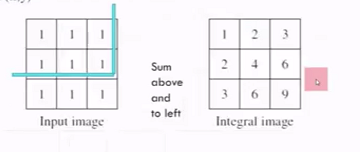
\includegraphics{./img1}
\caption{}
\label{fig:Capture}
\end{figure}

Integral image allows for the calculation of sum of all pixels inside any given rectangle using only four values at the corners of the rectangle.

\begin{figure}[h]
\centering
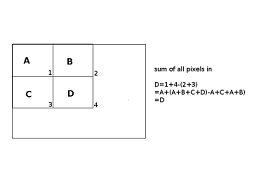
\includegraphics{./image1}
\caption{}
\label{fig:Image}
\end{figure}


\item Adaboost:--Adaboost is machine learning algorithm which helps in finding only the best features among all these 160,000+ features. After these features are found a weighted combination of all these features in use in evaluating and deciding any given window has a face or not.Each of the selected features are considered ok to be included if they can atleast perform better than random guessing(detects more than half cases).
These features are also called as weak classifiers. Adaboost constructs a strong classifier as a linear combination of these weak clssifiers.
\item Cascading:--If an image contains one or more faces it is obvious that an excessive large amount of the evaluated sub-windows would still be negetive(non-faces). So the algorithm should concentrate on discarding non-faces quickley and spend more time on preferable faces region. Hence a single classifier formed out of linear combination of all the best features are not good to evaluate due to coomputational cost. Therefore, the classifer is used which is composed of stages each containing a strong classifier. So all the features are grouped into several stages where each stage has certain number of features.The job of each stage is used to determine whether the given sub window is definitely not a face or may be a face.
\end{itemize}
\begin{thebibliography}{9}

\bibitem{lamport94}
  Face Detection,
  \emph{A Survey
Erik Hjelm�as1}.
 Department of Informatics, University of Oslo,
  norway.


\bibitem{lamport94}
 Detecting Faces in Images,
  \emph{A Survey
Ming-Hsuan Yang, Member, IEEE, David J. Kriegman, Senior Member, IEEE, and
Narendra Ahuja, Fellow}.
   IEEE.
 
\bibitem{lamport94}
  Robust Real-Time Face Detection,
  \emph{PAUL VIOLA}.
 Microsoft Research, One Microsoft Way, Redmond, WA 98052, USA,
 July 11, 2003.
 
  \bibitem{lamport94}
 Rapid Object Detection using a Boosted Cascade of Simple
Features,
  \emph{Paul Viola Michael Jones}.
 Mitsubishi Electric Research Labs Compaq CRL
201 Broadway, 8th FL One Cambridge Center
Cambridge,
  MA 02139 Cambridge, MA 02142.
 
 
\end{thebibliography}
\end{document}